\subsection{Overview}
Mossack Fonseca & Co. is a Panamanian law firm and corporate service provider, which is the world’s fourth biggest provider of offshore financial services. From its 1977 foundation until the April 2016 publication of the Panama Papers it remained mostly obscure, even though it sits at the heart of the global offshore industry, and acts for about 300,000 companies. More than half are registered in British tax havens – as well as in the UK. The firm received worldwide media attention in April 2016, when the International Consortium of Investigative Journalists published information about its clients' financial dealings in the Panama Papers articles, following the release of an enormous cache of its documents from between 1970 and 2015 leaked to the news media. The solution to the Panama Paper leak would be identifying the relationship among the nodes, and get valuable information
\subsection{Objective}
Establishing a network among the person behind The Panama Paper Leak, Power Law Network, Routing Network, Six Sigma. Using graph databases becomes increasingly popular in domains where data can be modeled as a set of connected objects. Graph databases enable to query such data using graph-based queries in a relatively simple manner in comparison to the classical relational databases. In this project, we will use graph database, Neo4j, to identify the network behind the top-notch chain of interlinked people behind the biggest leak of history, The Panama Paper Case Leak. Here, organizations would be considered as the node and the persons would be the relationship between the node. Further through machine learning algorithms we would study their relations and their effect on the society and produce our study output. As Machine learning is about analyzing data to ‘learn’ a model or using an algorithm that can be applied to make predictions on new data sets. These insights can be expressed as relationships between nodes in a graph. Graph databases enable efficient storage and traversal of information about relationships. Therefore, graph data would be the input of machine learning processing. To yield our study to a valuable conclusion.
\subsection{Challanges}

Working with 2.6TB of data is challanging because there is no machine and database is build to handle such a large amount of data. To achieve at our objective of establishing a network among the person behind The Panama Paper Leak, Power Law Network, Routing Network, Six Sigma.

\subsection{How you are going to achive the objective}
Firstly we will segregated the data as: Data contained in the Paradise Papers:
\begin{itemize}
\item Officer: a person or company who plays a role in an offshore entity
\item Offshore: made, situated, or registered abroad, especially in order to take advantage of lower taxes or costs or less stringent regulation.
\item Intermediary: go-between for someone seeking an offshore corporation and an offshore service provider — usually a law-firm or a middleman that asks an offshore service provider to create an offshore firm for a client. 
\item	Entity: a company, trust or fund created in a low-tax, offshore jurisdiction by an agent. 
\item	Address: postal address as it appears in the original databases obtained by ICIJ. 
\item	Other: additional information items.
\end{itemize}
Then we will achieve the objective by applying predicting analysis, routing and establish a network among the nodes associated in the Panama Paper Leak.

\subsubsection{Tools}
Neo4j, a NoSQL database provides a mechanism for storage and retrieval of data that is modelled in means other than the tabular relations used in relational databases. Motivations for this approach include: simplicity of design, simpler "horizontal" scaling to clusters of machines (which is a problem for relational databases), and finer control over availability. The data structures used by NoSQL databases (e.g. key-value, wide column, graph, or document) are different from those used by default in relational databases, making some operations faster in NoSQL

\subsubsection{Technique}
Need a comparison b/w the alternative The particular suitability of a given NoSQL database depends on the problem it must solve. In theoretical computer science, the CAP theorem, also named Brewer's theorem after computer scientist Eric Brewer, states that it is impossible for a distributed data store to simultaneously provide more than two out of the following three guarantees. No distributed system is safe from network failures, thus network partitioning generally has to be tolerated. In the presence of a partition, one is then left with two options: consistency or availability. When choosing consistency over availability, the system will return an error or a time-out if particular information cannot be guaranteed to be up to date due to network partitioning. When choosing availability over consistency, the system will always process the query and try to return the most recent available version of the information, even if it cannot guarantee it is up to date due to network partitioning. Most NoSQL stores lack true ACID transactions, although a few databases, such as MarkLogic, Aerospike, FairCom c-treeACE, Google Spanner (though technically a NewSQL database), Symas LMDB, and OrientDB have made them central to their designs.

\subsection{Time line}

\begin{figure}[h]
\centering
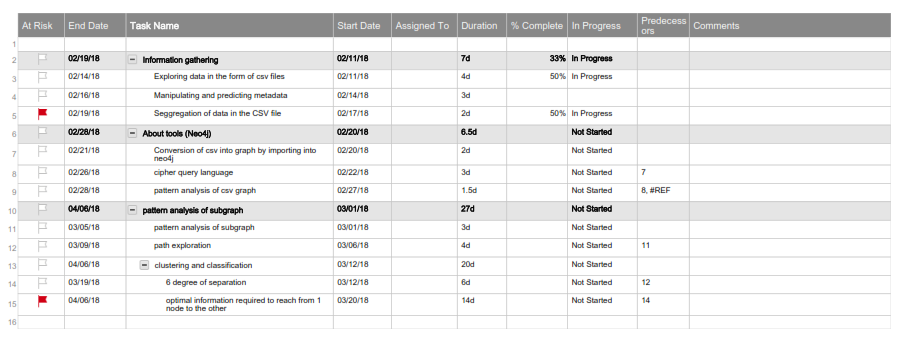
\includegraphics[width=\textwidth]{images/timeline.png}
\caption{Time-Line}
\end{figure}


\begin{figure}[h]
\centering
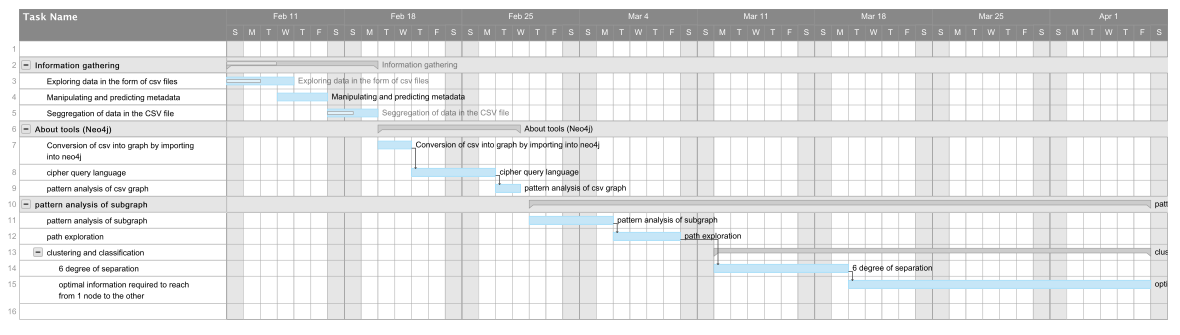
\includegraphics[width=\textwidth]{images/gantt-chart.png}
\caption{Gantt-Chart}
\end{figure}

\newpage

\subsection{What are the possible challanges to achive the objective}
Applying different types of attribute in clustering analysis such as interval-scaled variables, binary variables, nominal, ordinal and ratio variables to the variables of mixed type.

\subsection{Contribution of the group members}
\subsubsection{Anwesha Sinha}

\begin{itemize}
    \item Analyzing the new features and bring it into the project.
    \item Thinking Creatively towards the project.
    \item Managing new changes in the project.
\end{itemize}

\subsubsection{Geetanshu Mathur}

\begin{itemize}
    \item Managing the overall time-line of the project.
    \item Bringing in new features to the project.
    \item Keep all the team members motivated.
\end{itemize}

\subsubsection{Suyesh Mathur}
\begin{itemize}
    \item Keeping the things up-to date w.r.t time-line.
    \item Reporting any flaw or fault seen in overall progress/process of the project.
    \item Keeping the record of every discussion related to the project in safe repository.
\end{itemize}